\chapter{Autofunciones y Espectros de autovalores OSMC (Capítulo 6)} \label{cap:transition_apendice}

\subsection*{Caso A ($\text{Ri}_b=0\text{.}04$)}


\begin{figure}[H]
  \centering
    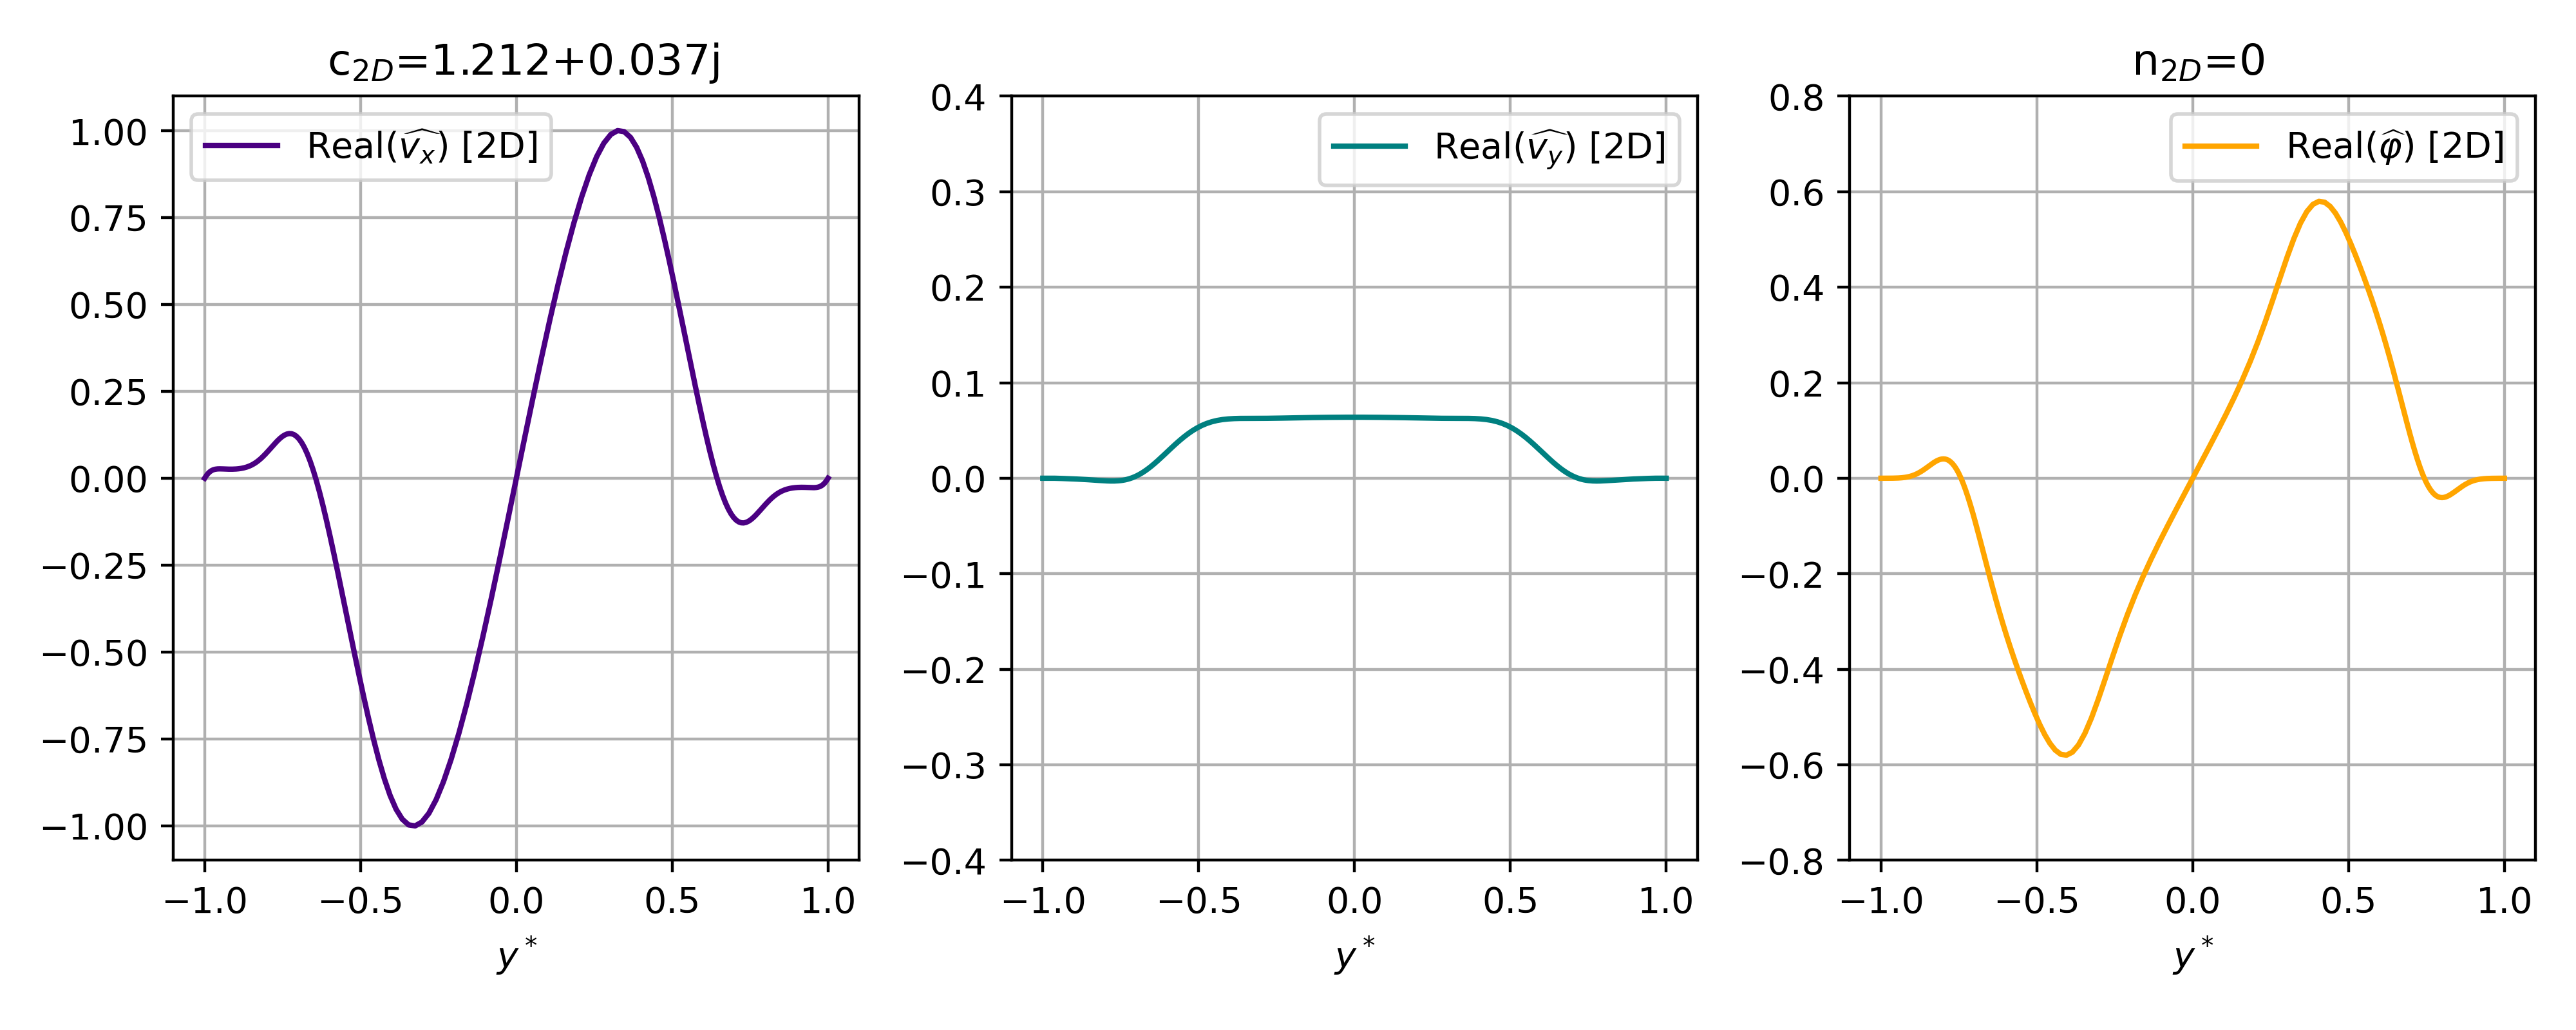
\includegraphics[width=\textwidth]{figures/apendices/transicion/Re5000-Ri1Em6-Pr071_eigenfun_AC1-AC4.png}
  \caption{Autofunciones 2D de los ensayos A-C1, A-C2, A-C3 y A-C4.}
  \label{fig:eigenfuns1-Re5000-Pr071}
\end{figure}

\begin{figure}[H]
  \centering    
    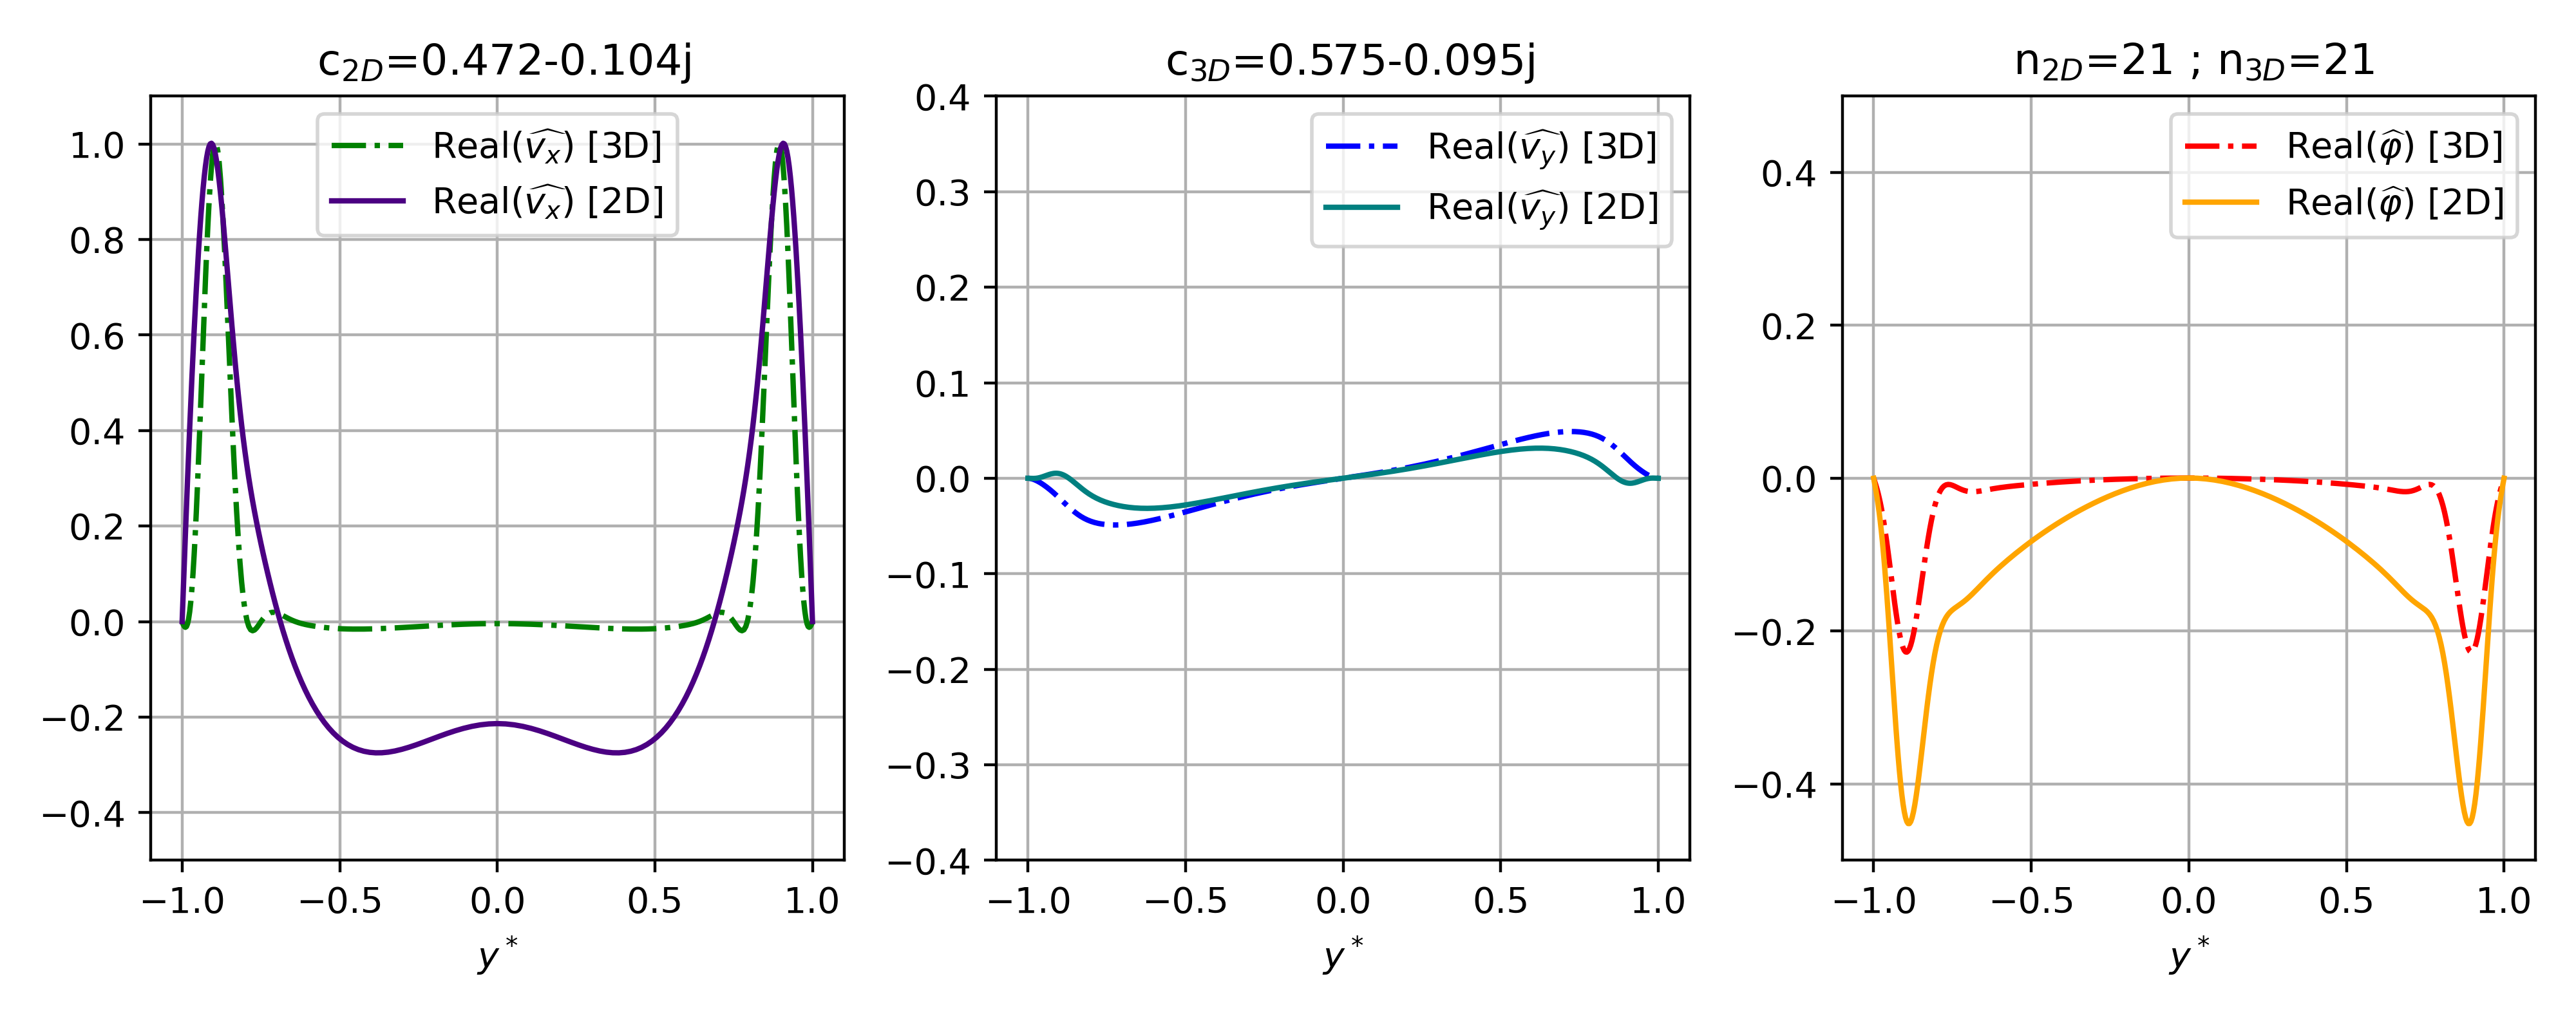
\includegraphics[width=\textwidth]{figures/apendices/transicion/Re5000-Ri1Em6-Pr071_eigenfun_AC7_AC9.png}
  \caption{Autofunciones 2D y 3D de los ensayos A-C7 y A-C9.}
  \label{fig:eigenfuns2-Re5000-Pr071}
\end{figure}

\begin{figure}[H]
  \centering  
    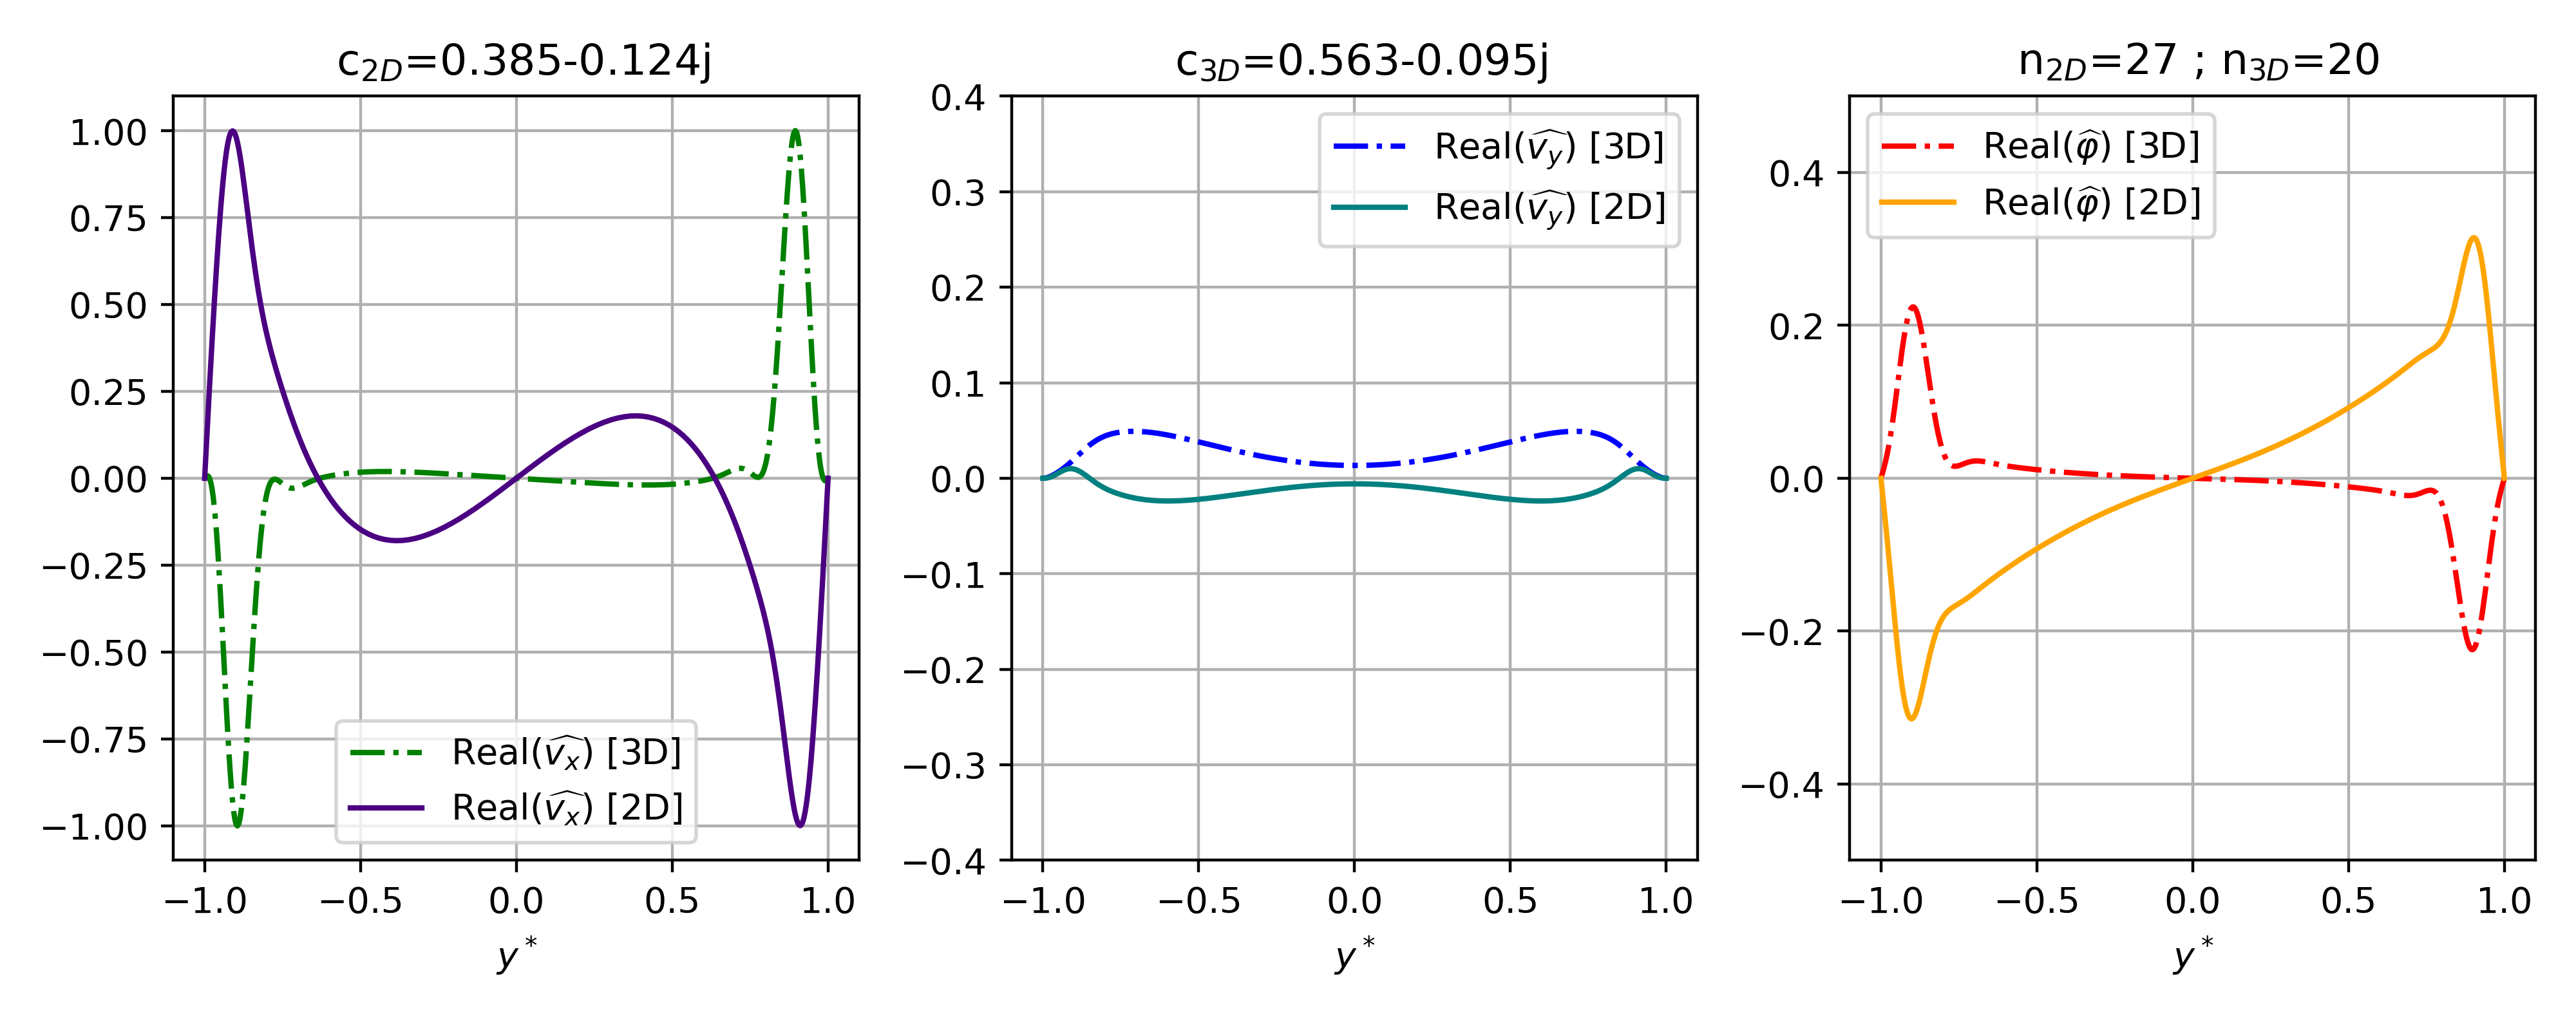
\includegraphics[width=\textwidth]{figures/apendices/transicion/Re5000-Ri1Em6-Pr071_eigenfun_AC8_AC10.png}
  \caption{Autofunciones 2D y 3D de los ensayos A-C8 y A-C10.}
  \label{fig:eigenfuns3-Re5000-Pr071}
\end{figure}

\begin{figure}[H]
  \centering
    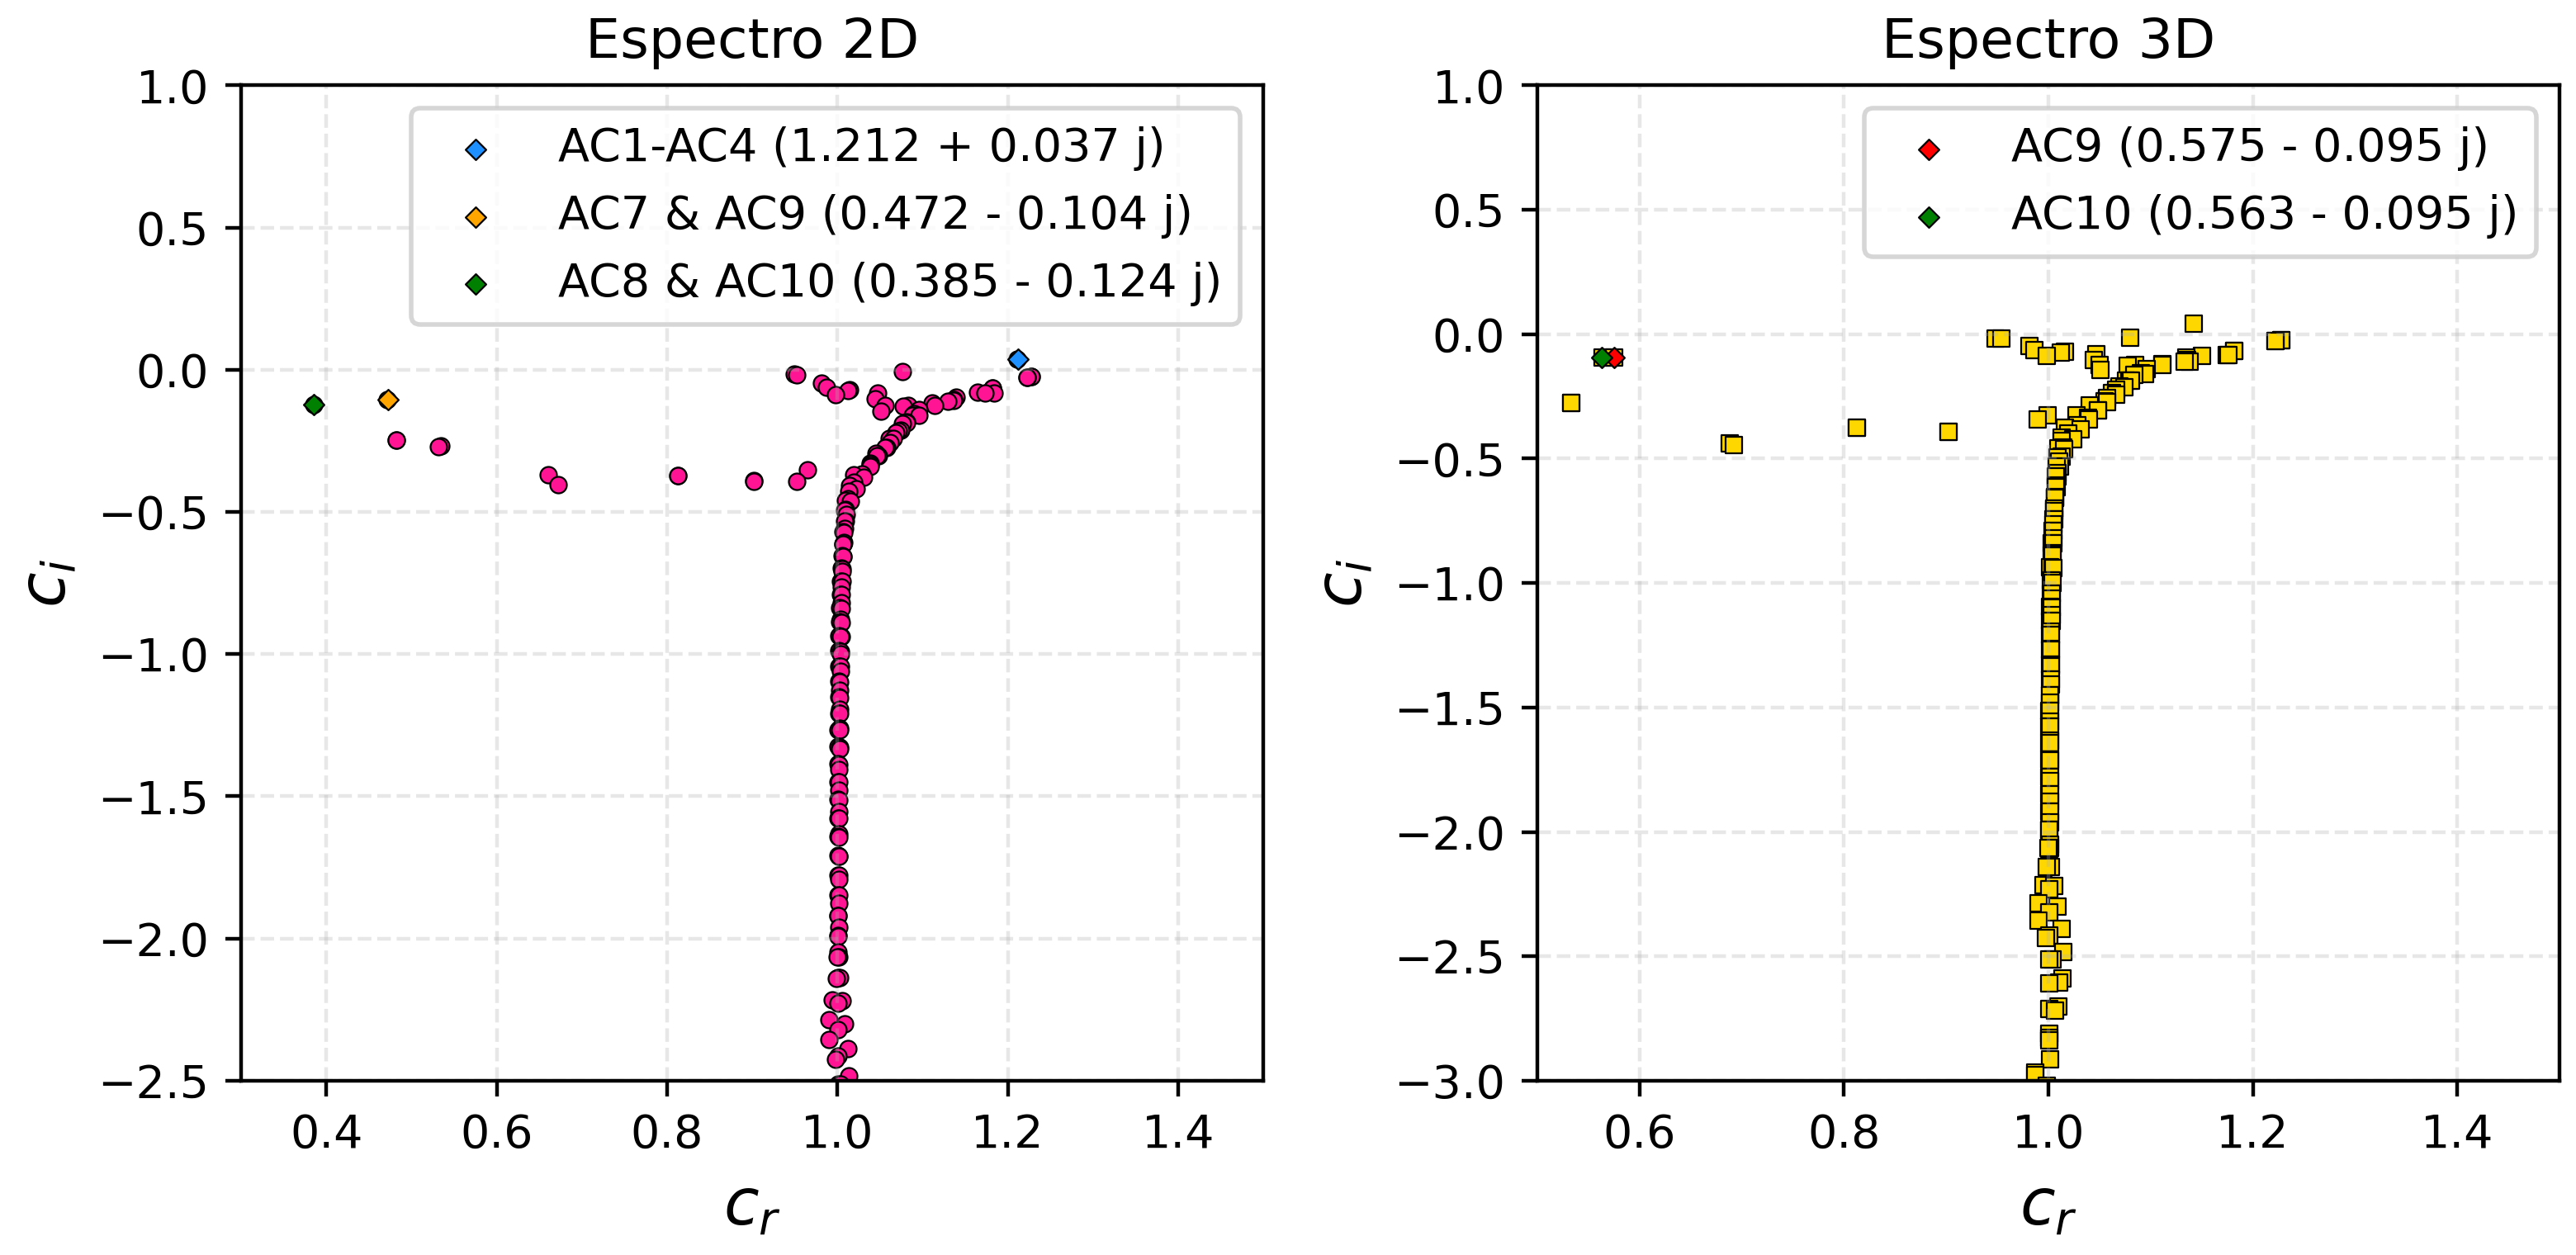
\includegraphics[width=\textwidth]{figures/apendices/transicion/Re5000-Pr071-Ri1Em6_eigenvals.png}
  \caption{Espectros de autovalores 2D y 3D ($\text{Ra}=65$).}
  \label{fig:spectra-Re5000-Pr0071}
\end{figure}

\newpage

\subsection*{Caso B ($\text{Ri}_b=1\text{.}06$)}


\begin{figure}[H]
  \centering
    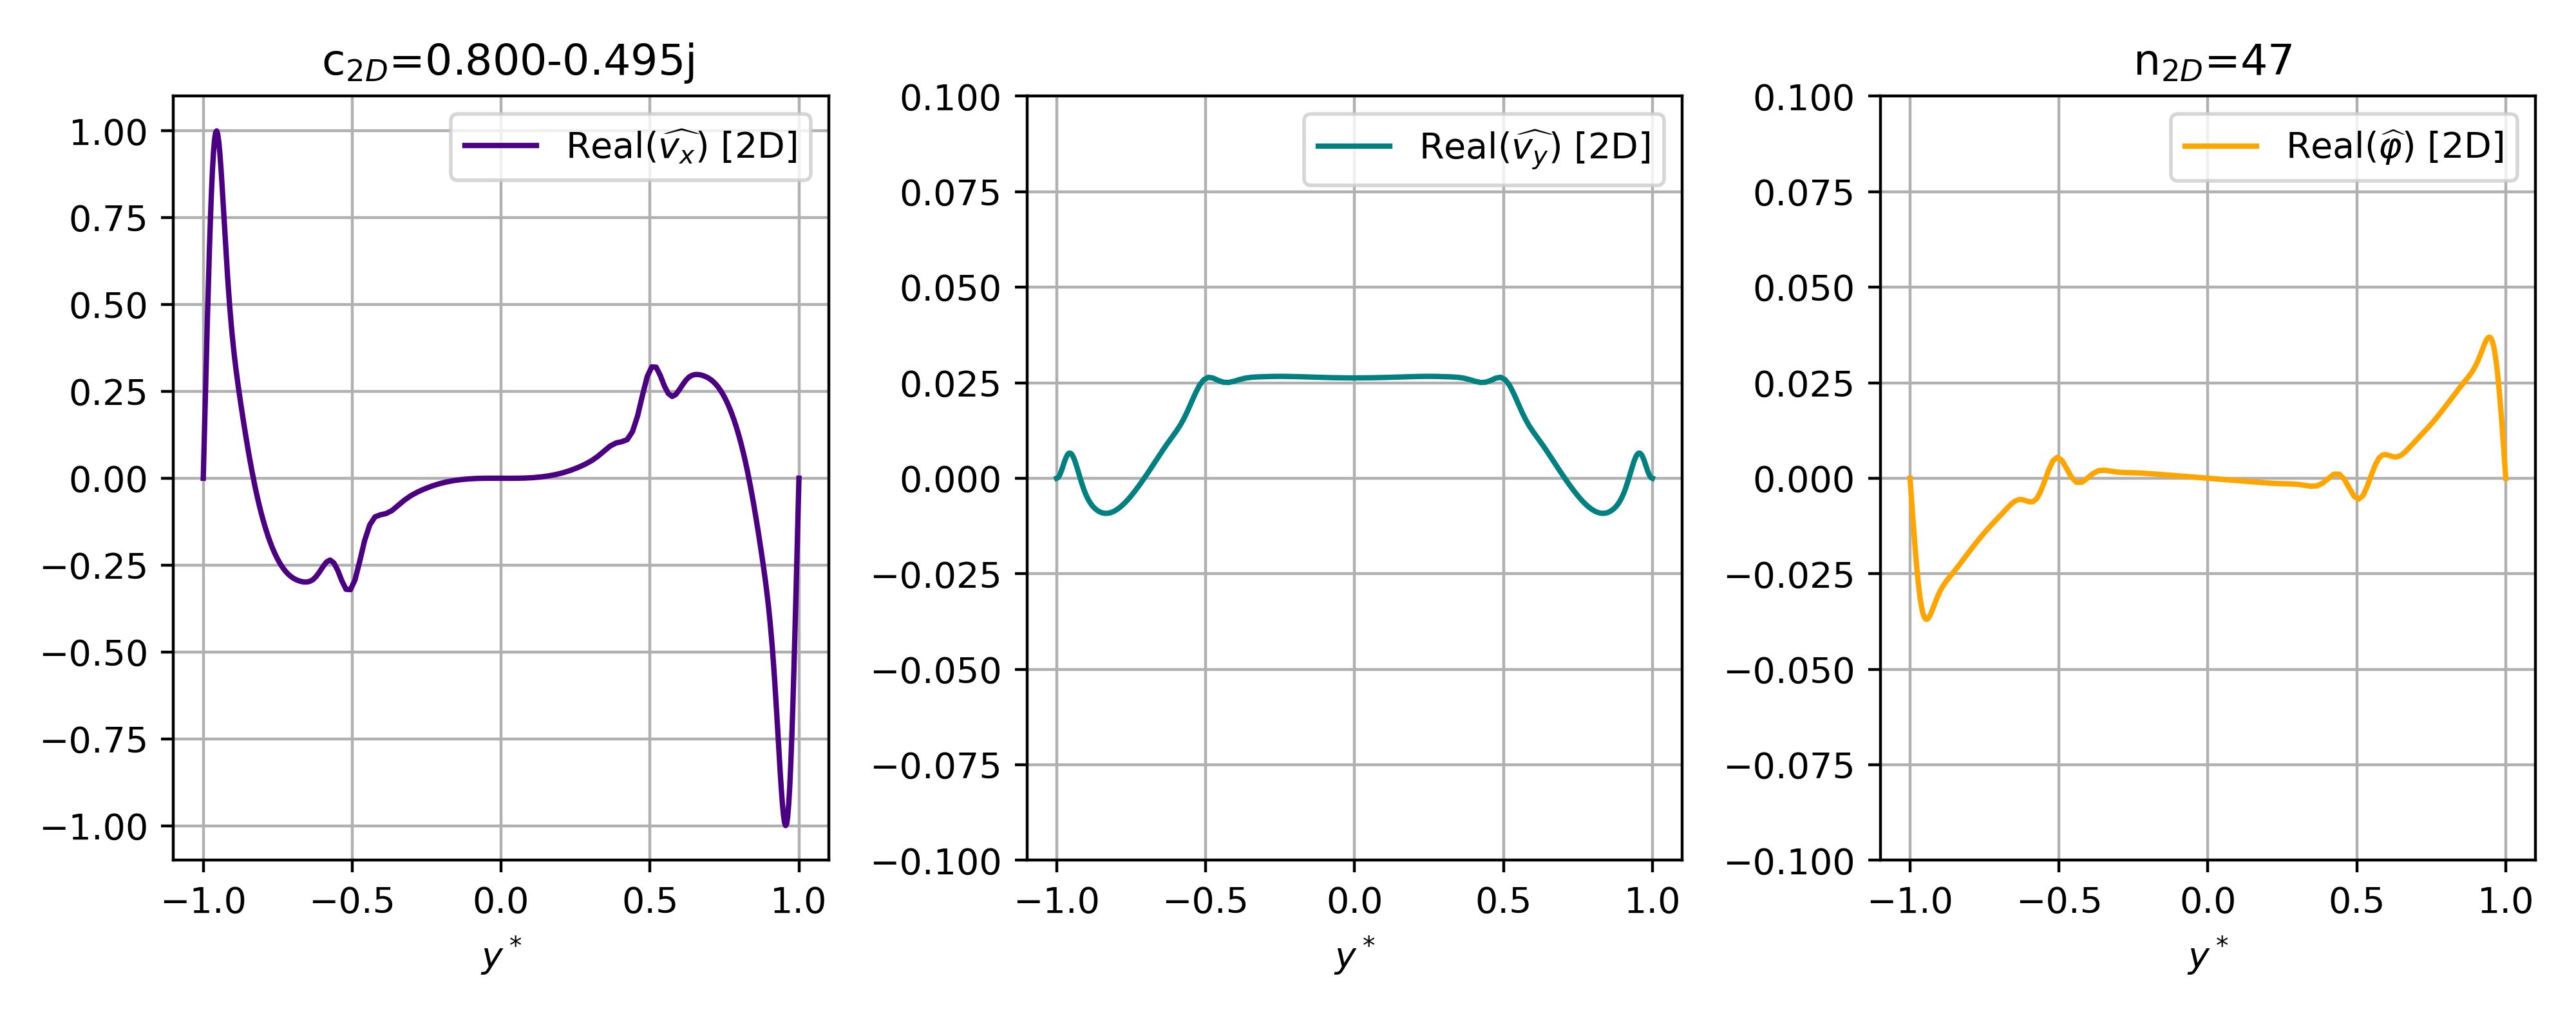
\includegraphics[width=\textwidth]{figures/apendices/transicion/Re5000-Ri1Em4-Pr071_eigenfun_BC2.png}
  \caption{Autofunciones 2D del ensayo B-C2.}
  \label{fig:eigenfuns1-Re5000-Pr071}
\end{figure}

\begin{figure}[H]
  \centering    
    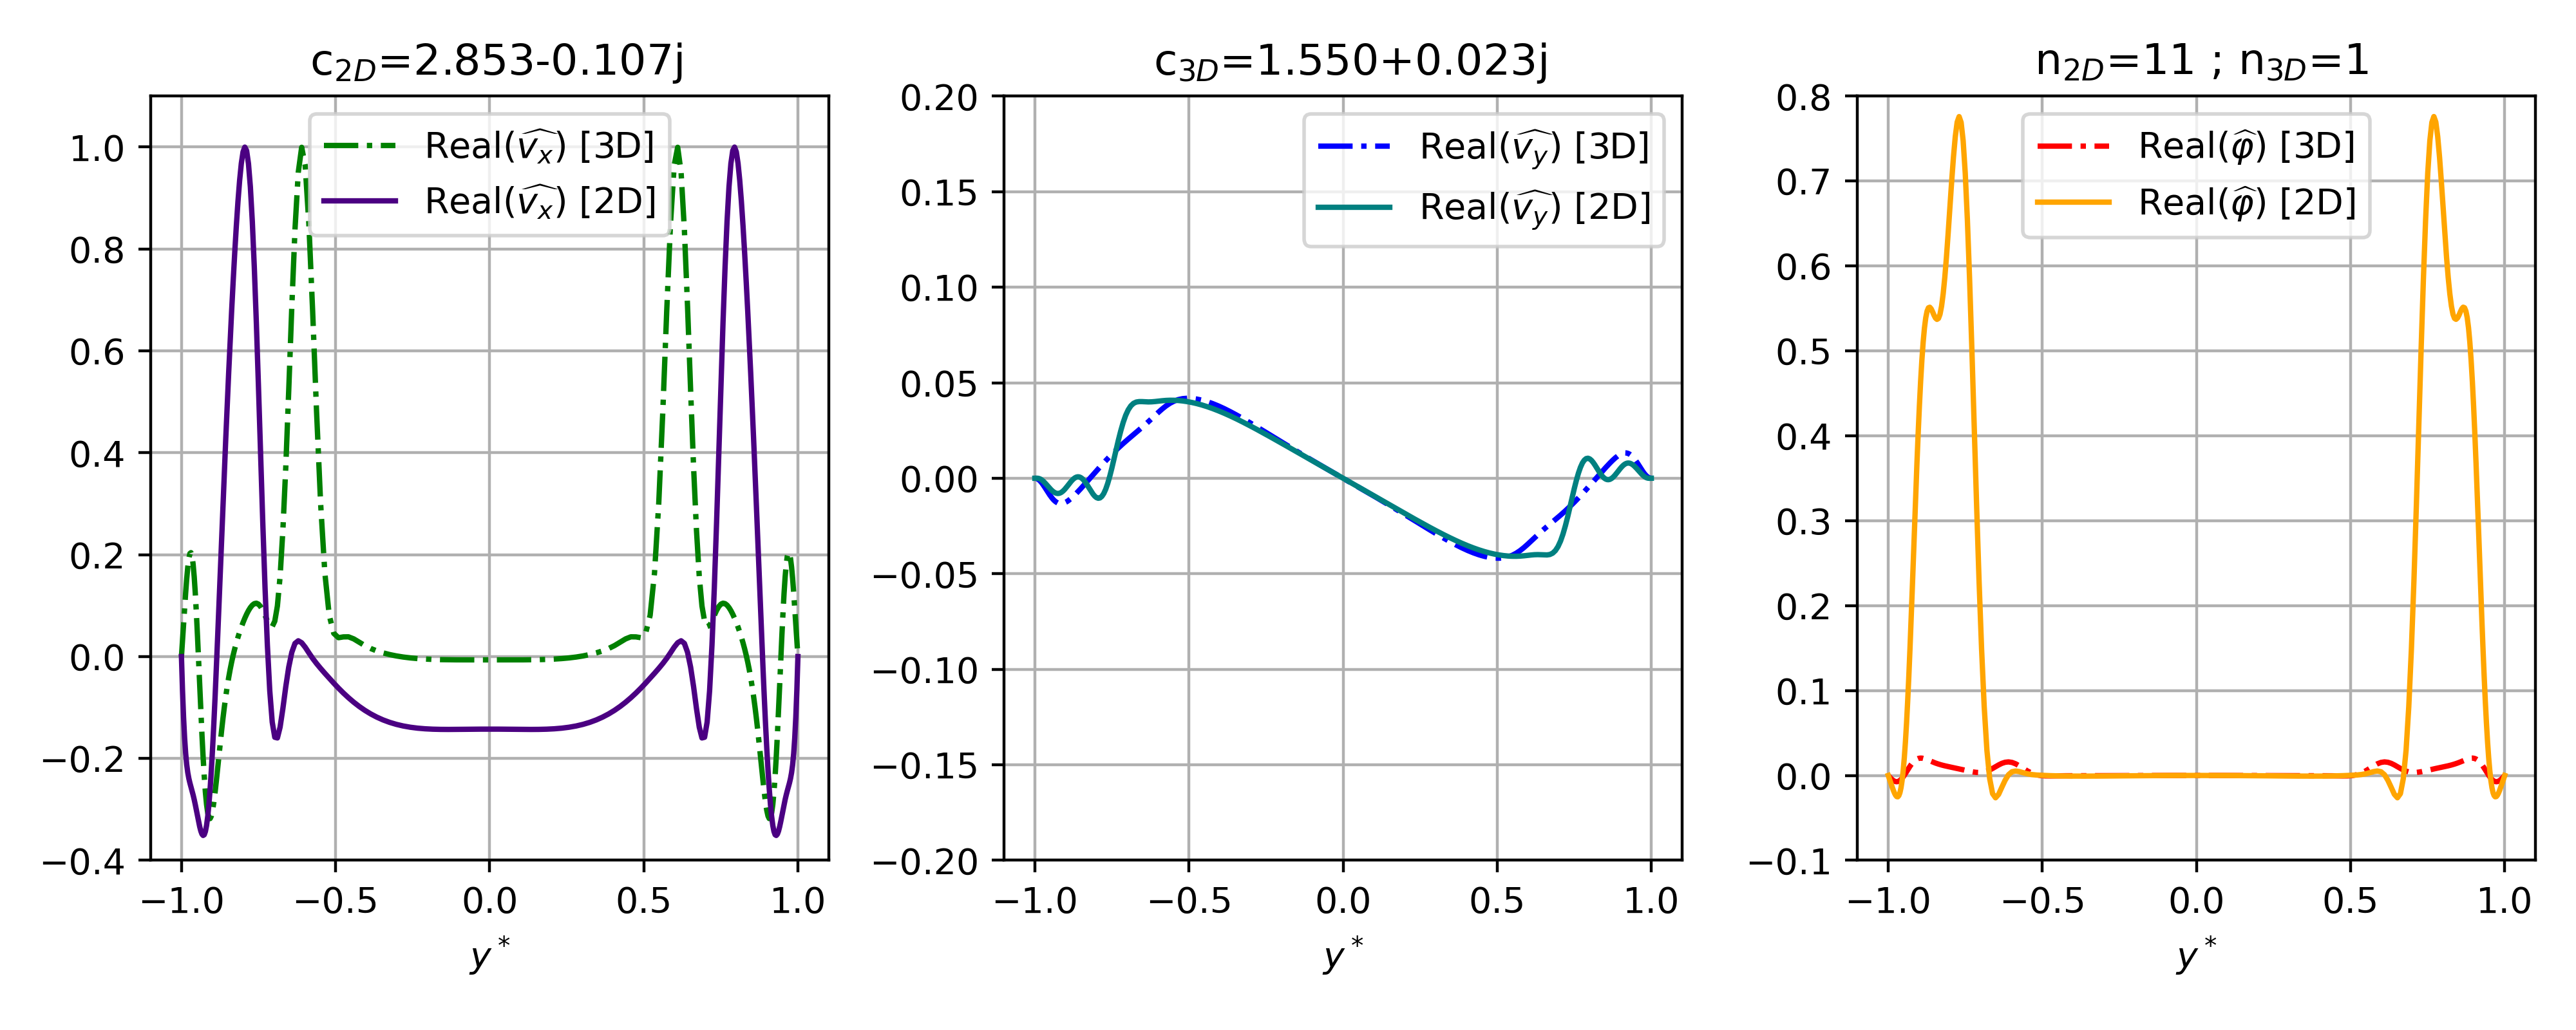
\includegraphics[width=\textwidth]{figures/apendices/transicion/Re5000-Ri1Em4-Pr071_eigenfun_BC3_BC5.png}
  \caption{Autofunciones 2D y 3D de los ensayos B-C3 y B-C5.}
  \label{fig:eigenfuns2-Re5000-Pr071}
\end{figure}

\begin{figure}[H]
  \centering  
    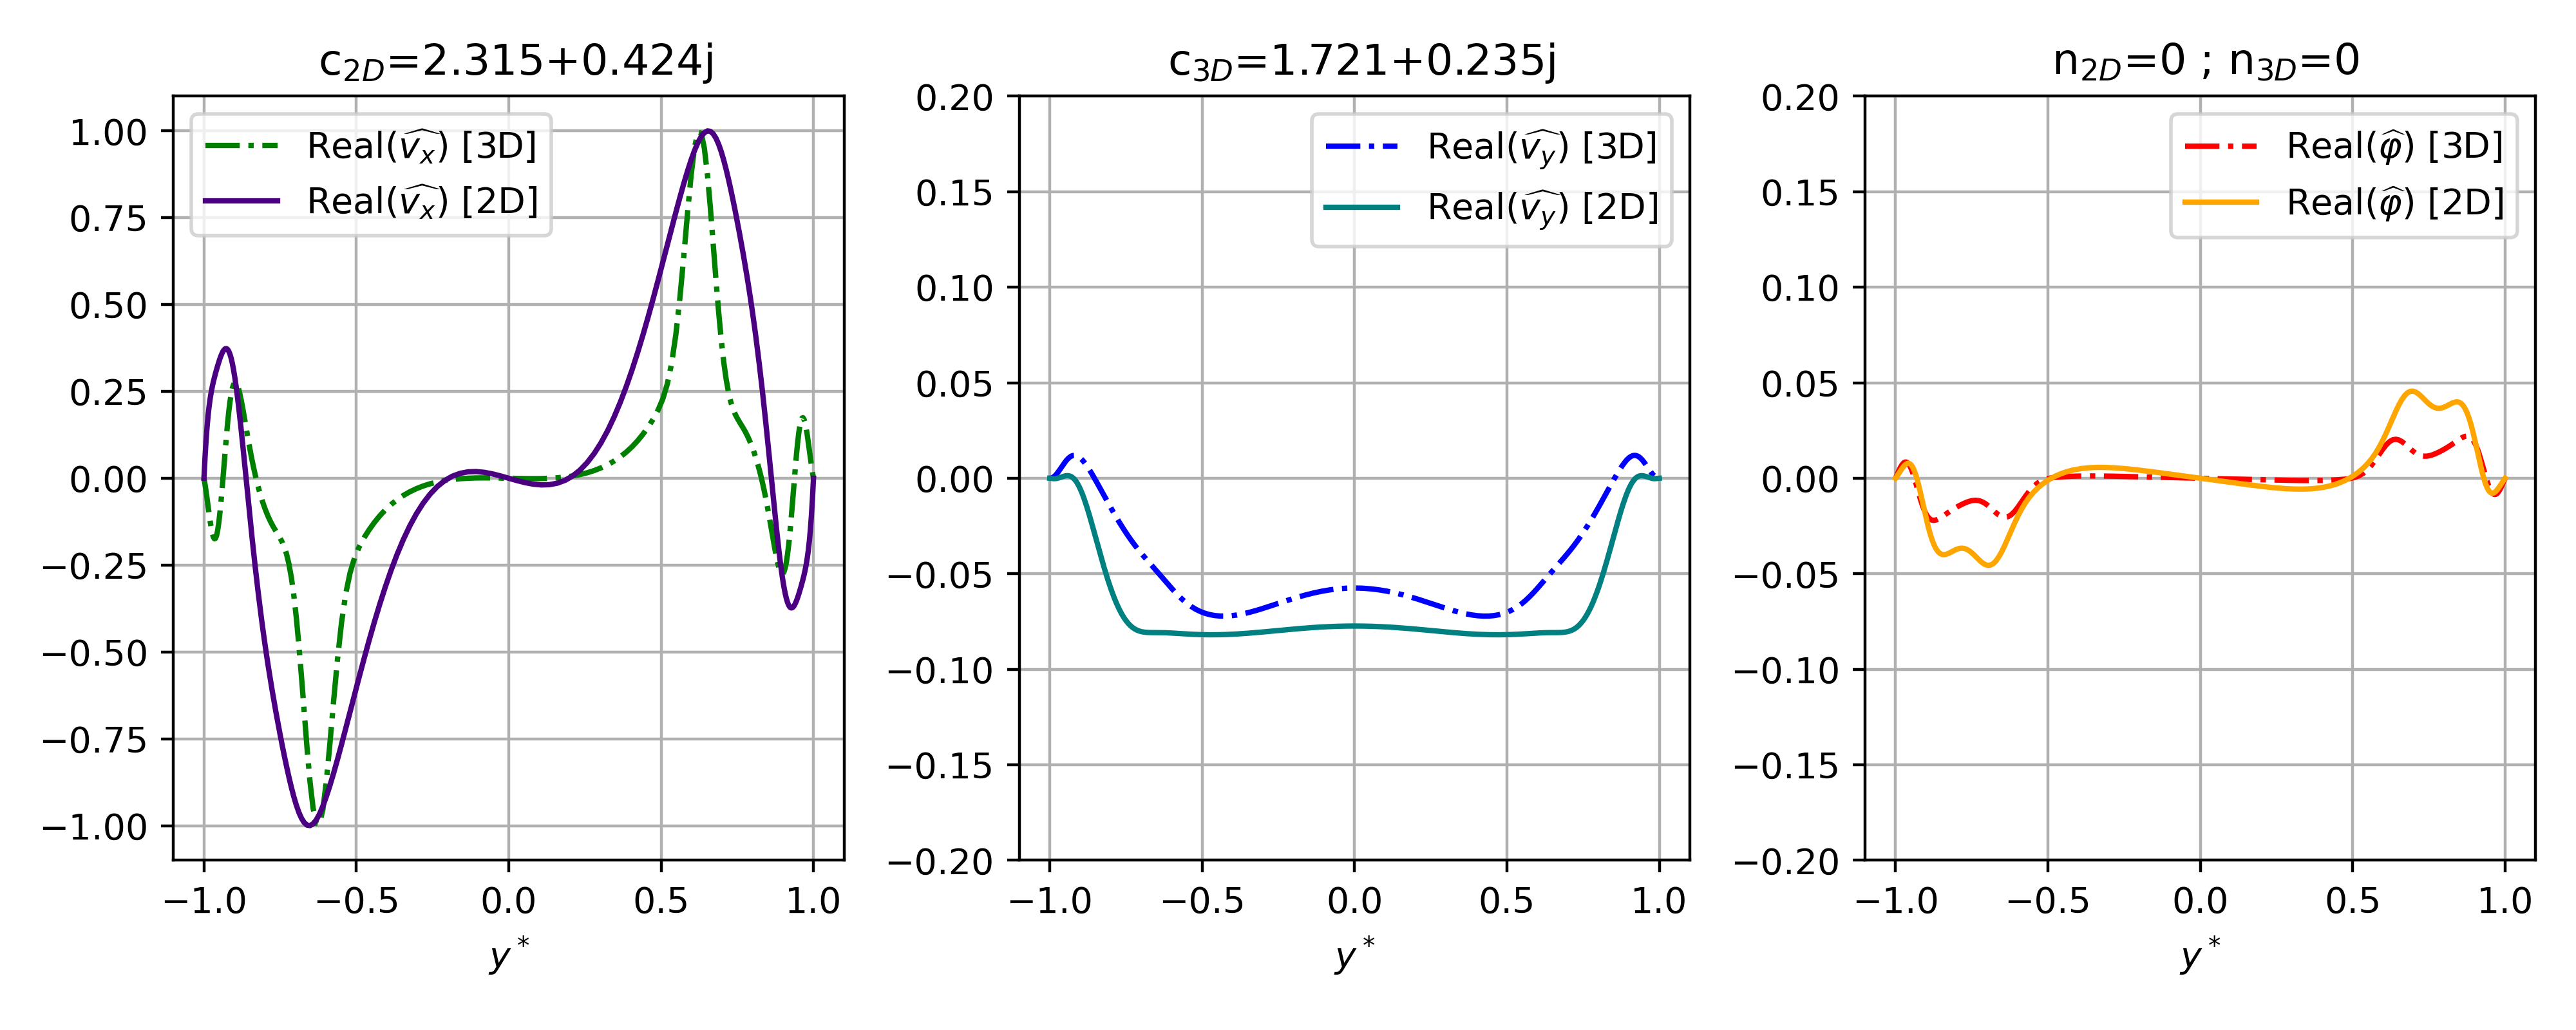
\includegraphics[width=\textwidth]{figures/apendices/transicion/Re5000-Ri1Em4-Pr071_eigenfun_BC4.png}
  \caption{Autofunciones 2D y 3D del ensayo B-C4.}
  \label{fig:eigenfuns3-Re5000-Pr071}
\end{figure}

\begin{figure}[H]
  \centering
    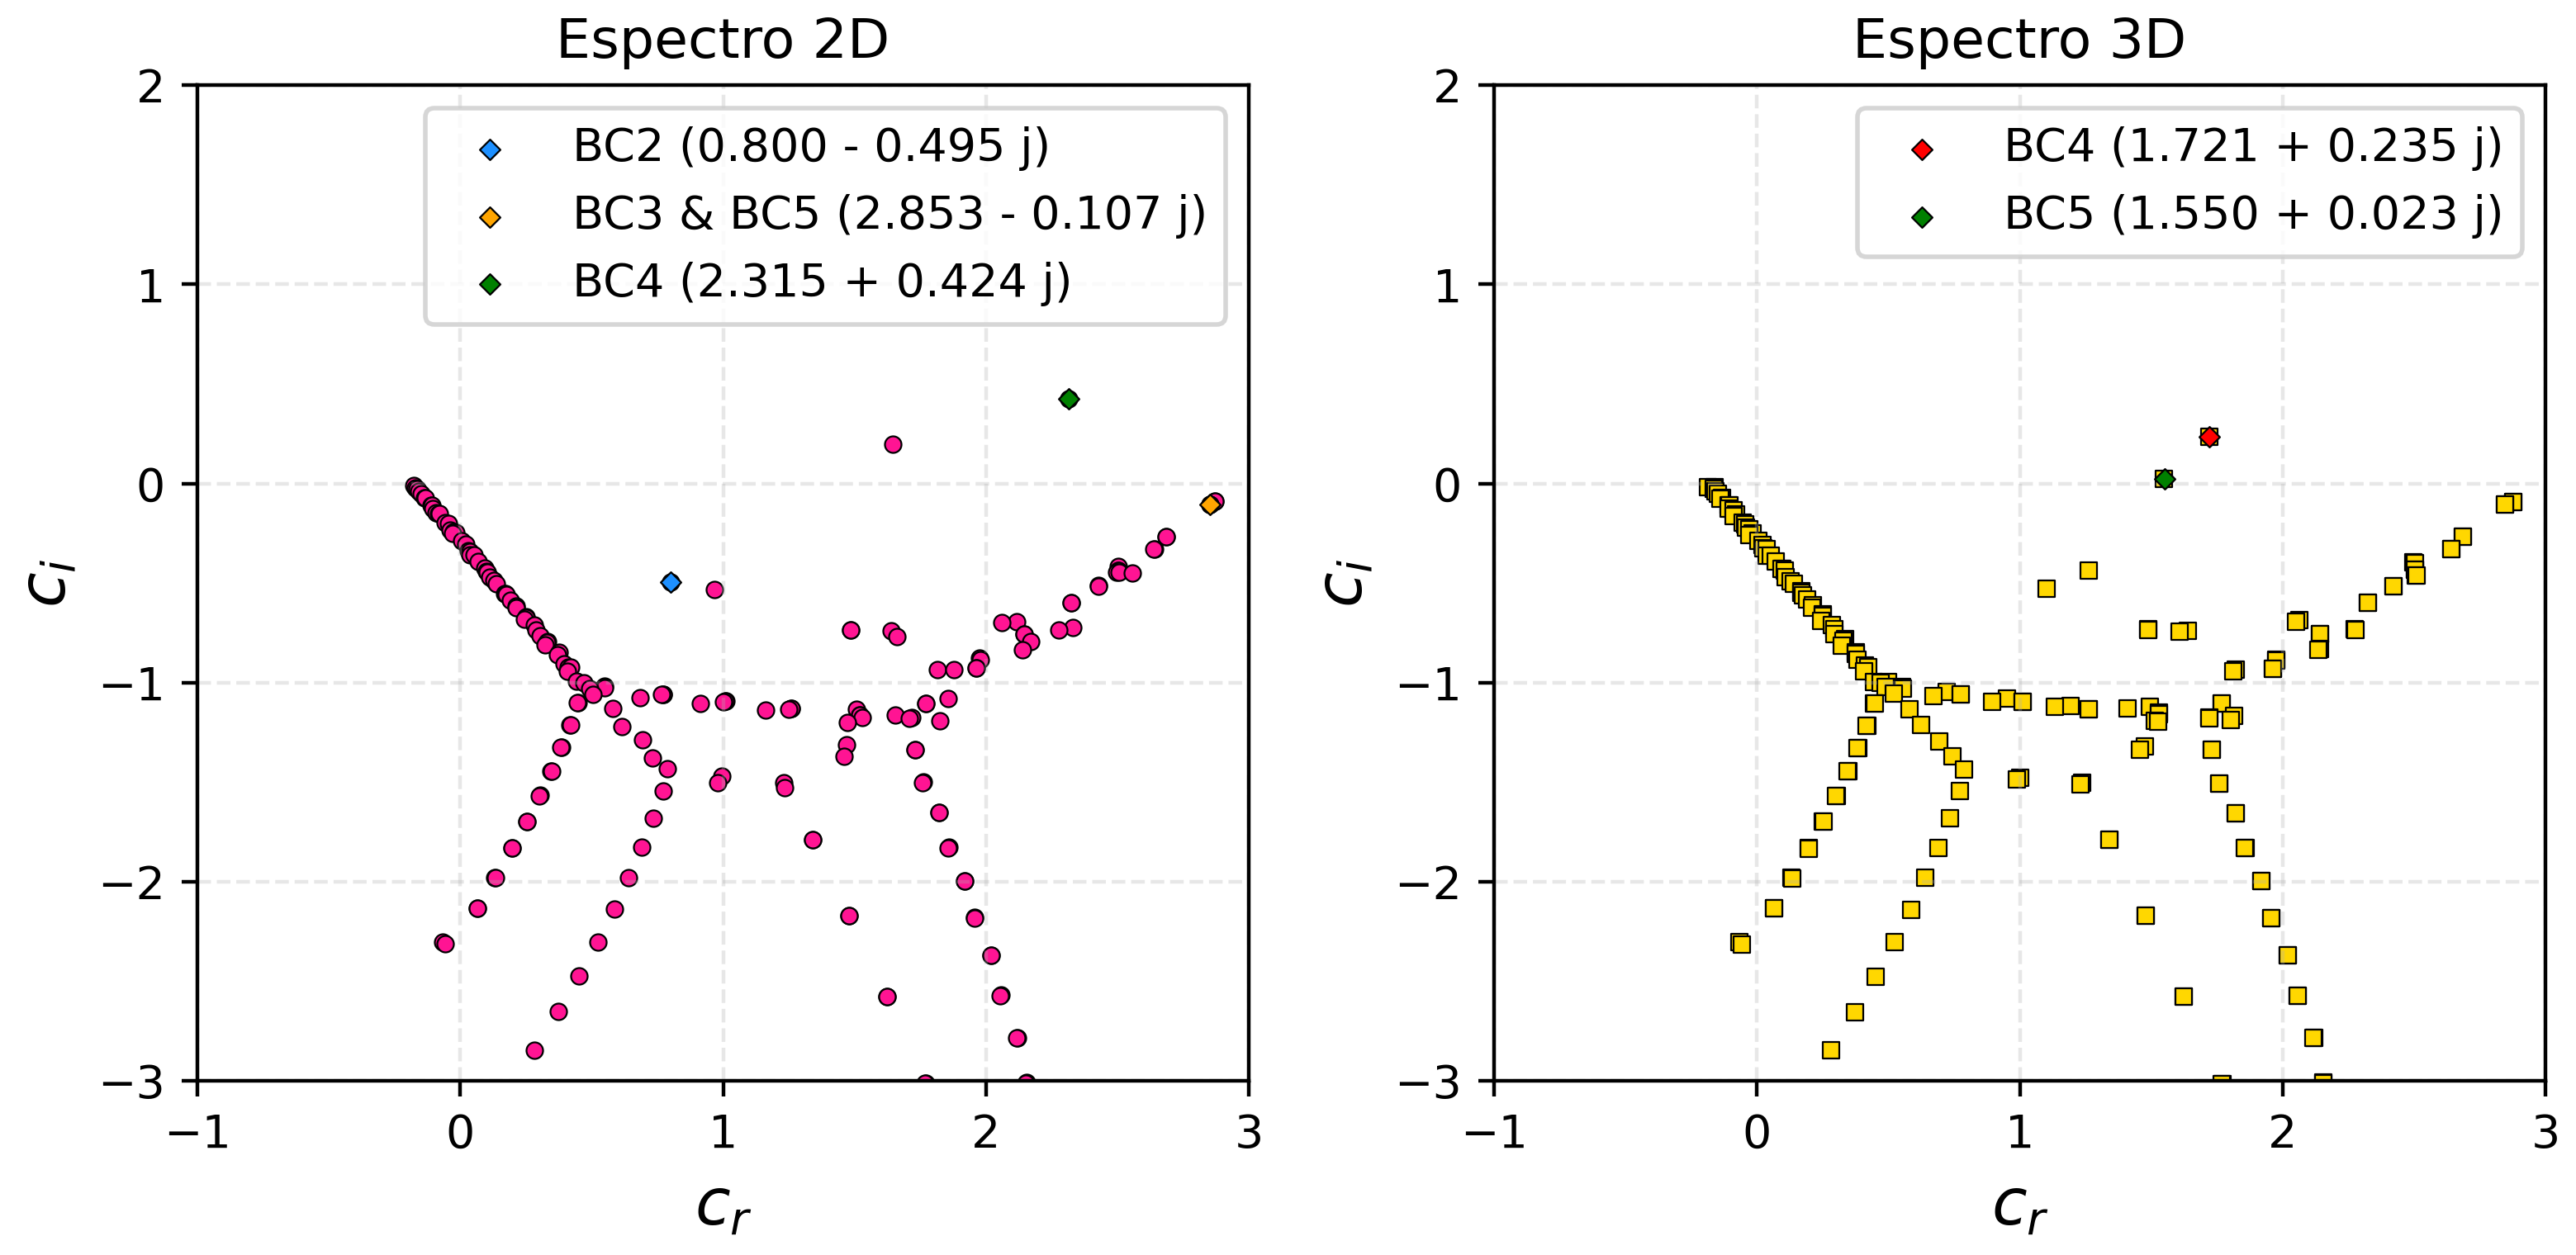
\includegraphics[width=\textwidth]{figures/apendices/transicion/Re5000-Pr071-Ri1Em4_eigenvals.png}
  \caption{Espectros de autovalores 2D y 3D ($\text{Ra}=1775$).}
  \label{fig:spectra-Re5000-Pr0071}
\end{figure}



